\documentclass[portrait,final,a0paper]{baposter}
%\documentclass[a4shrink,portrait,final]{baposter}
% Usa a4shrink for an a4 sized paper.

\tracingstats=2

% special 
\usepackage{ifthen}
\usepackage{ifpdf}
\usepackage{float}
\usepackage{color}

% fonts
\usepackage{latexsym}
\usepackage{amsmath} 
\usepackage{amssymb} 
\usepackage{bm}
\usepackage{wasysym}


\ifpdf
\usepackage{graphicx}
\usepackage{epstopdf}
\else
\usepackage{graphicx}
\usepackage{epsfig}
\fi


\graphicspath{{figures/},{PROG/figures/}}


%%%%%%%%%%%%%%%%%%%%%%%%%%%%%%%%%%%%%%%%%%%%%%%%%%%%%%%%%%%%%%%%


% NEW 
\newcommand{\abs}[1]{\left|#1\right|}
\newcommand{\Prob}{\mbox{Prob}\,}
\newcommand{\erf}{\mbox{erf}\,}
\newcommand{\barline}[1]{#1}

% math symbols I
\newcommand{\sinc}{\mbox{sinc}}
\newcommand{\const}{\mbox{const}}
\newcommand{\trc}{\mbox{trace}}
\newcommand{\intt}{\int\!\!\!\!\int }
\newcommand{\ointt}{\int\!\!\!\!\int\!\!\!\!\!\circ\ }
\newcommand{\ar}{\mathsf r}
\newcommand{\im}{\mbox{Im}}
\newcommand{\re}{\mbox{Re}}

% math symbols II
\newcommand{\eexp}{\mbox{e}^}
\newcommand{\bra}{\left\langle}
\newcommand{\ket}{\right\rangle}

% Mass symbol
\newcommand{\mass}{\mathsf{m}} 
\newcommand{\Mass}{\mathsf{M}} 

% more math commands
\newcommand{\tbox}[1]{\mbox{\tiny #1}}
\newcommand{\bmsf}[1]{\bm{\mathsf{#1}}} 
%\newcommand{\amatrix}[1]{\matrix{#1}} 
\newcommand{\amatrix}[1]{\begin{matrix} #1 \end{matrix}} 
\newcommand{\pd}[2]{\frac{\partial #1}{\partial #2}}

% equations
\newcommand{\mylabel}[1]{\label{#1}} 
%\newcommand{\mylabel}[1]{\textcolor{blue}{[#1]}\label{#1}} 
\newcommand{\beq}{\begin{eqnarray}}
\newcommand{\eeq}{\end{eqnarray}} 
\newcommand{\be}[1]{\begin{eqnarray}\ifthenelse{#1=-1}{\nonumber}{\ifthenelse{#1=0}{}{\mylabel{e#1}}}}
\newcommand{\ee}{\end{eqnarray}} 

% arrangement
\newcommand{\drawline}{\begin{picture}(500,1)\line(1,0){500}\end{picture}}
\newcommand{\bitem}{$\bullet$ \ \ \ }
\newcommand{\Cn}[1]{\begin{center} #1 \end{center}}
\newcommand{\mpg}[2][1.0\hsize]{\begin{minipage}[b]{#1}{#2}\end{minipage}}
\newcommand{\mpgt}[2][1.0\hsize]{\begin{minipage}[t]{#1}{#2}\end{minipage}}
\newcommand{\putgraph}[2][width=0.30\hsize]{\includegraphics[#1]{#2}}

% more
%\newcommand{\Eq}[1]{Eq.\!\!~(\ref{#1})}
%\newcommand{\Fig}[1]{Fig.\!\!~\ref{#1}}  
\newcommand{\Eq}[1]{\textcolor{blue}{Eq.\!\!~(\ref{#1})}} 
\newcommand{\Fig}[1]{\textcolor{blue}{Fig.}\!\!~\ref{#1}} 
\newcommand{\hide}[1]{} %{\textcolor{red}{[hidden text]}} %{}
\newcommand{\rmrk}[1]{\textcolor{red}{#1}}


%%%%%%%%%%%%%%%%%%%%%%%%%%%%%%%%%%%%%%%%%%%%%%%%%%%%%%%%%%%%%%%%%%%%%%%%%%%

% extra math commands by jarondl
\newcommand{\inner}[2]{\left \langle #1 \middle| #2\right\rangle} % Inner product
\newcommand{\avgangle}[1]{\left\langle #1 \right\rangle} % Average <x>

%fminipage using fancybox package
\newenvironment{fminipage}%
  {\begin{Sbox}\begin{minipage}}%
  {\end{minipage}\end{Sbox}\fbox{\TheSbox}}

%%%%%%%%%%%%%%%%%%%%%%%%%%%%%%%%%%%%%%%%%%%%%%%%%%%%%%%%%%%%%%%%%%%%%%%%%%%%%%
%%% Begin of Document
%%%%%%%%%%%%%%%%%%%%%%%%%%%%%%%%%%%%%%%%%%%%%%%%%%%%%%%%%%%%%%%%%%%%%%%%%%%%%%

\begin{document}

%%%%%%%%%%%%%%%%%%%%%%%%%%%%%%%%%%%%%%%%%%%%%%%%%%%%%%%%%%%%%%%%%%%%%%%%%%%%%%
%%% Here starts the poster
%%%---------------------------------------------------------------------------
%%% Format it to your taste with the options
%%%%%%%%%%%%%%%%%%%%%%%%%%%%%%%%%%%%%%%%%%%%%%%%%%%%%%%%%%%%%%%%%%%%%%%%%%%%%%
% Define some colors
\definecolor{silver}{cmyk}{0,0,0,0.3}
\definecolor{yellow}{cmyk}{0,0,0.9,0.0}
\definecolor{reddishyellow}{cmyk}{0,0.22,1.0,0.0}
\definecolor{black}{cmyk}{0,0,0.0,1.0}
\definecolor{darkYellow}{cmyk}{0,0,1.0,0.5}
\definecolor{darkSilver}{cmyk}{0,0,0,0.1}

\definecolor{lightyellow}{cmyk}{0,0,0.3,0.0}
\definecolor{lighteryellow}{cmyk}{0,0,0.1,0.0}
\definecolor{lighteryellow}{cmyk}{0,0,0.1,0.0}
\definecolor{lightestyellow}{cmyk}{0,0,0.05,0.0}

%%
%\background{
%  \begin{tikzpicture}[remember picture,overlay]%
%    \draw (current page.north west)+(-2em,2em) node[anchor=north west] {\includegraphics[height=1.1\textheight]{silhouettes_background}};
%  \end{tikzpicture}%
%}
\typeout{Poster Starts}

\begin{poster}%
  % Poster Options
  {
  bgColorOne=lightgray!30,
  %bgColorTwo=yellow,
  headerheight=0.1\textheight,
  columns=3,
  headershade=plain,
  headerColorOne=green!40,
  boxColorOne=lightgray!75,
  headershape=smallrounded,
  textborder=roundedsmall,
  linewidth=0.5pt,
  borderColor=green,
  headerborder=open,
  eyecatcher=false,
  background=plain
}
  % Eye Catcher
  {\includegraphics[width=10em]{D1077}} % No eye catcher for this poster. (eyecatcher=no above). If an eye catcher is present, the title is centered between eye-catcher and logo.
  % Title
  {\sf 
Transport in 1D and 2D:\\ 
From linear response to effective range hopping.
  }
  % Authors
  {\sf
  \vspace{2em}  Yaron de Leeuw,  BGU
  }
  % University logo
  {\hspace{10em}
\includegraphics[width=20em]{BGU}\
  }

  \tikzstyle{light shaded}=[top color=baposterBGtwo!30!white,bottom color=baposterBGone!30!white,shading=axis,shading angle=30]


%%%%%%%%%%%%%%%%%%%%%%%%%%%%%%%%%%%%%%%%%%%%%%%%%%%%%%%%%%%%%%%%%%%%%%%%%%%%%%
%%% Now define the boxes that make up the poster
%%%---------------------------------------------------------------------------
%%% Each box has a name and can be placed absolutely or relatively.
%%% The only inconvenience is that you can only specify a relative position 
%%% towards an already declared box. So if you have a box attached to the 
%%% bottom, one to the top and a third one which should be in between, you 
%%% have to specify the top and bottom boxes before you specify the middle 
%%% box.
%%%%%%%%%%%%%%%%%%%%%%%%%%%%%%%%%%%%%%%%%%%%%%%%%%%%%%%%%%%%%%%%%%%%%%%%%%%%%%


%%%%%%%%%%%%%%%%%%%%%%%%%%%%%%%%%%%%%%%%%%%%%%%%%%%%%%%%%%%%%%%%%%%%%%%%%%%%%%
  \headerbox{The model}{name=model,column=0,row=0}{
%%%%%%%%%%%%%%%%%%%%%%%%%%%%%%%%%%%%%%%%%%%%%%%%%%%%%%%%%%%%%%%%%%%%%%%%%%%%%%
{}

We consider 1D or 2D network systems whose dynamics is described
by a rate equation, with transitions rates $w_{nm}$ that form a symmetric matrix.
In particular (but no exclusively) we are interested
in a model where the rates depend exponentially on the distance
between randomly distributed sites, namely $w_{nm}\propto \exp(|x_n-x_m|/\xi)$.
It is natural to characterize such a system by a sparsity parameter~$s$
that reflects the connectivity of the network. In the above example
the natural definition is $s=\xi/r_0$ where $r_0$ is the average distance
between neighboring sites.
}
%%%%%%%%%%%%%%%%%%%%%%%%%%%%%%%%%%%%%%%%%%%%%%%%%%%%%%%%%%%%%%%%%%%%%%%%%%%%%%
  \headerbox{Diffusion coefficient}{name=diffusion,column=0, below=model}{
%%%%%%%%%%%%%%%%%%%%%%%%%%%%%%%%%%%%%%%%%%%%%%%%%%%%%%%%%%%%%%%%%%%%%%%%%%%%%%
{}

Our interest is focused in the diffusion coefficient $D$ that characterizes the
long time dynamics of a spreading distribution. In 1D it is well known that $D$ can display an abrupt
percolation-like transition from diffusive (${D>0}$) to sub-diffusive (${D=0}$)
behavior as the sparsity parameter drops below the critical value ${s_c=1}$.  
The question arises whether such a transition happens also in
higher dimensions.

There are two major routes in developing 
a theory for~$D$. It may be deduced  from spectral properties ,
but one may also try to find ways to evaluate it directly
via a resistor network calculation.
The extension of the resistor network method to wide distributions, leads to a generalized Variable Range Hopping (VRH) strategy.
In what follows we pursue the same direction and obtain an
improved Effective Range Hopping (ERH) estimate for~$D$.
Using this approach we show that in the 2D case, as $s$ becomes small,
the functional $D[\bm{w}]$ exhibits a smooth crossover from LRT behavior 
to semi-linear VRH-like dependence.  
 }

%%%%%%%%%%%%%%%%%%%%%%%%%%%%%%%%%%%%%%%%%%%%%%%%%%%%%%%%%%%%%%%%%%%%%%%%%%%%%%
  \headerbox{The $1d$ chain model}{name=lrt,column=0,below=diffusion}{
%%%%%%%%%%%%%%%%%%%%%%%%%%%%%%%%%%%%%%%%%%%%%%%%%%%%%%%%%%%%%%%%%%%%%%%%%%%%%%
{} In the $1d$ chain model, the location of each site has a uniform random distribution on a $1d$ line.

The rates are calculated according to $w_{nm} = w_0 \exp(-|r_m-r_n|/\xi)$, with only nearest neighbor transitions
($b=1$). We can convert the spacing distribution to rate distribution, and, making the analogy with adding connectors in series, we obtain:
\beq
D = D[w_n] = \left( \frac{1}{N} \sum_n \frac{1}{w_n} \right)^{-1} 
 =  \frac{s-1}{s} \, w_0
\eeq
for $s>1$, with $s=\xi/r_0$. For $0<s<1$, there is a sub diffusive regime, where the survival probability and spreading are:
\beq
S(t) \ \ &\propto& \ \ t^{2s/(1+s)}   \\ 
\mathcal{P}(t) \ \ &\propto& \ \ t^{-s/(1+s)}
\eeq
 These are exact analytic results, based on work by Shlomo Alexander\cite{alexander}, and they are summed up in panel (a) of figure \ref{fig:alexander}.
  \vspace{0.3em}
  }

%%%%%%%%%%%%%%%%%%%%%%%%%%%%%%%%%%%%%%%%%%%%%%%%%%%%%%%%%%%%%%%%%%%%%%%%%%%%%%
  \headerbox{Diffusion as a function of sparsity}{name=alexander,column=1,span=2,row=0}{
%%%%%%%%%%%%%%%%%%%%%%%%%%%%%%%%%%%%%%%%%%%%%%%%%%%%%%%%%%%%%%%%%%%%%%%%%%%%%%
{}  

\begin{figure}[H]
  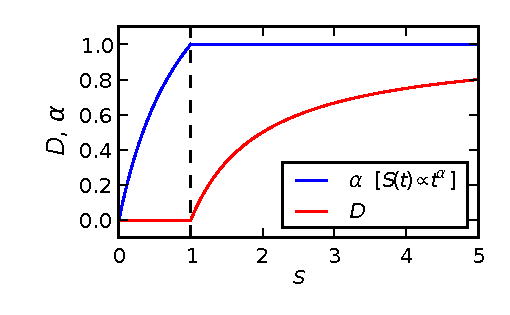
\includegraphics[width=0.45\textwidth]{alexander}
  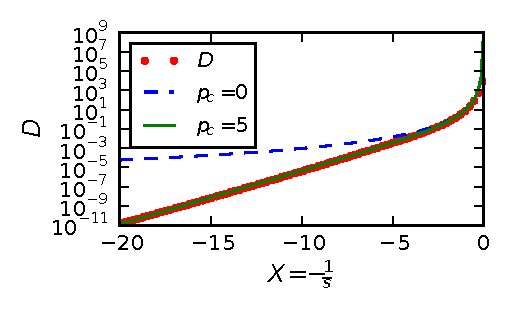
\includegraphics[width=0.45\textwidth]{ERH}
\caption{Theoretical results for a $1d$ chain model, contrasting the $2d$ results. In the $1d$ plot, on the left, the blue line is the power of the spreading. It shows a sub-diffusive regime where $0<s<1$, and a diffusive regime for $s>1$. The red line is of the diffusion coefficient $D$, which is zero for the sub-diffusive regime $s<1$. It is dimensionless as we set $r_0=1$. In the $2d$ plot, on the right, we see the diffusion coefficient, numerical fit results vs ERH, as explained in sections \ref{sec:diff2d} and \ref{sec:num_d_2d}. The $Y$ axis is $D$ in logarithmic scale, while the $X$ axis is $X=-1/s$. The dots are numerical fit results, extracted from plots such as \ref{fig:exp_2d_D_vs_subD}. The dashed line is of the LRT result, and the solid line is the ERH result with $p_c = 5$.}
\label{fig:alexander}
\end{figure}

  \vspace{0.3em}
  }


%%%%%%%%%%%%%%%%%%%%%%%%%%%%%%%%%%%%%%%%%%%%%%%%%%%%%%%%%%%%%%%%%%%%%%%%%%%%%%
  \headerbox{Linear response}{name=lrt,column=1,below=alexander}{
%%%%%%%%%%%%%%%%%%%%%%%%%%%%%%%%%%%%%%%%%%%%%%%%%%%%%%%%%%%%%%%%%%%%%%%%%%%%%%
If we had an ordered lattice, then the exact result for $D$ would be 
%
\beq
D  =  D_{\tbox{LRT}}[\bm{w}]   =  \frac{1}{2d}\iint w(r,\epsilon) \ r^2  \ \rho(r,\epsilon) \ d\epsilon dr 
\eeq
%
This expression is strictly {\em linear}.
For the infinite temperature variation of 2D random site model we get  
%
\beq
D \ \ = \ \ 3\pi \, s^4 \, w_0
\eeq
%
This expression will not work for ${s<1}$ because sparse contribution 
of strongly coupled sites do not contribute to the transport. 
Only percolating trajectories do have a contribution. We are therefore urged 
to introduce approximation schemes that takes this connectivity 
issue into account.  
 
}
%%%%%%%%%%%%%%%%%%%%%%%%%%%%%%%%%%%%%%%%%%%%%%%%%%%%%%%%%%%%%%%%%%%%%%%%%%%%%%
  \headerbox{Spectral Analysis}{name=spect,column=2,below=alexander}{
%%%%%%%%%%%%%%%%%%%%%%%%%%%%%%%%%%%%%%%%%%%%%%%%%%%%%%%%%%%%%%%%%%%%%%%%%%%%%%

In a diffusive system the coarse grained spreading 
is described by the standard diffusion equation,
with an evolving Gaussian distribution  
%  
\beq
\rho(x;t) \ \ = \ \ \prod_{i=1}^d \frac{1}{\sqrt{2\pi}\sigma(t)} 
\exp\left[-\frac{1}{2}\left(\frac{x_i}{\sigma(t)}\right)^2 \right]
\eeq
%
where $\sigma^2=2Dt$. It follows from this expression that 
% 
\beq
S(t) \ \ = \ \ \left\langle r^2(t) \right\rangle  \ \ = \ \ (2d)Dt
\eeq
%
and 
%
\beq
\mathcal{P}(t) \quad \approx \quad  \frac{1}{\left({4\pi D t}\right)^{d/2}} 
\qquad\qquad[r_0^d=1]
\eeq
%
The eignevalues of the diffusion equation are $\lambda=Dq^2$ 
where the possible values of the momentum are determined  
by the periodic boundary conditions as $q=(2\pi/L)\vec{n}$. 
It follows that the cumulative number of eigenstates is  
%
\beq \label{eq:expected_D_2d}
\mathcal{N}(\lambda) \ \ = \ \ 
\int_0^\lambda g(\lambda')d\lambda' \quad 
= \quad \left(\frac{L}{2\pi}\right)^d
\frac{\Omega_d}{d}
\left[\frac{\lambda}{D}\right]^{d/2}
\eeq



It is well known that the survival probability 
is related to the eigenvalues of $\bm{w}$ through the relation
%
\beq \label{eq:survival}
\mathcal{P}(t) \ \ = \ \ \frac{1}{N}\sum_\lambda \eexp{\lambda t} \ \ \equiv \ \ \int_0^{\infty} g(\lambda)d\lambda \ \eexp{\lambda t}
\eeq
%
For a diffusive system one can verify that the 
indeed the expressions above 
for $g(\lambda)$ and $\mathcal{P}(t)$ 
are related by a Laplace transform.  
%
More generally, it follows that $D$ can be deduced from 
the asymptotic behavior of $g(\lambda)$
in the ${\lambda\rightarrow 0}$ limit  
where the diffusive description is valid.
%
In contrast to that for large $\lambda$ we expect $g(\lambda)$ to coincide 
with the distribution of the decay rates $\gamma_n=\sum_{m}w_{mn}$, 
reflecting localized modes.

}
%%%%%%%%%%%%%%%%%%%%%%%%%%%%%%%%%%%%%%%%%%%%%%%%%%%%%%%%%%%%%%%%%%%%%%%%%%%%%%
  \headerbox{Eigenvalue distributions}{name=eigvals,column=1,span=2,above=bottom}{
%%%%%%%%%%%%%%%%%%%%%%%%%%%%%%%%%%%%%%%%%%%%%%%%%%%%%%%%%%%%%%%%%%%%%%%%%%%%%%
%%%%%%%%%%%%%%%%%%5
\begin{figure}[H]
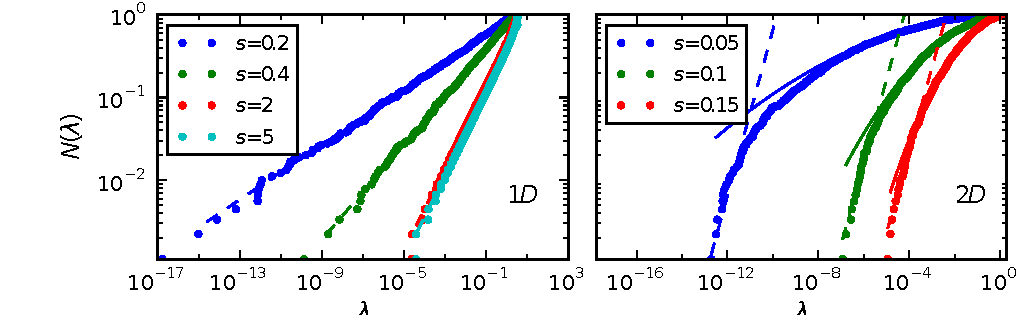
\includegraphics[clip, width=0.95\textwidth]{two_panels}
\caption{ $1D$ and $2D$ cummulative eigenvalue distribution, 
for several values of $s$.
 The dots represent numerical diagonalization. The dashed lines are the expected diffusion results according to \eqref{eq:expected_D_2d}, with $D$ as a fit parameter. The solid lines are according to Ariel's result, as presented in \eqref{eq:amir_expected} . There is a striking difference between the $1d$ and $2d$ cases. For $1d$, the slope for sparse models ($s<1$) is less than $\frac{1}{2}$, meaning we have sub-diffusion. In the $2d$ case, the low-$\lambda$ slope is always $1$, which correspondes to normal diffusion.} \label{fig:exp_2d_D_vs_subD}
\end{figure}
}

%%%%%%%%%%%%%%%%%%%%%%%%%%%%%%%%%%%%%%%%%%%%%%%%%%%%%%%%%%%%%%%%%%%%%%%%%%%%%%
  \headerbox{References}{name=references,column=2,above=bottom}{
%%%%%%%%%%%%%%%%%%%%%%%%%%%%%%%%%%%%%%%%%%%%%%%%%%%%%%%%%%%%%%%%%%%%%%%%%%%%%%

  \begin{thebibliography}{99}
  \bibitem{alexander}
    S. Alexander, J. Bernasconi, W. R. Schneider, R. Orbach, 
    Rev. Mod. Phys. 53, 175 (1981).


  \end{thebibliography}
  }


\end{poster}

\end{document}
